%!TEX root = ../document.tex
\section[Implementation Ideas (Author: Lauritz Thamsen)]{Implementation Ideas} \label{sec:IMPLEMENTATION_IDEAS}
%Lauritz
As described in Section~\ref{sec:PAPER_PROTOTYPE} and \ref{sec:FINAL_PROTOTYPE}, our proposed environment always presents relevant Data Contexts when the developer interacts with a statement.
Just like in a debugger, for example when the developer, hovers over an identifier in the application code, the IDE responds with actual data, either objects or database rows.
However, in contrast to ordinary debugging environments, a developer should not only be able to view the current state and step through the execution, but also add and evaluate statements.
This allows for an interactive style of development centered around seeing the impact and effects of code and queries immediately.
In order for such features to function properly, availability of runtime data needs to be ensured.
First, a developer can only see values and database entries for identifiers, if such data is available.
Second, statements that might or might not embed queries require referred variables and potentially even a database to run.
A realization of our idea would, therefore, implement components that gather the necessary data contexts from actual program runs as well as components that support developers in selecting interesting data contexts during development.

\subsection{Gathering Data Contexts}

Our approach depends on the availability of Data Contexts for the code sections of interest to the developer.
Such Data Contexts need to be realistic and immediately available to be useful.
Given these premises, we think of two approaches to provide Data Contexts for specific code sections:
Either deterministic test runs establish Data Contexts on demand or traces of the application's execution record Data Contexts in advance.
Running tests to provide the runtime during development would only require to store coverage information that associates code sections with test cases. Recording contextual information in advance would, however, imply storing as much data as necessary to actually run any statements in the sources of an application.
The time necessary for test execution depends on the granularity of the covering tests with a full spectrum from fine-grained, isolated unit tests to high-level, long-running acceptance tests.
Previously recorded Data Contexts, however, need just to be fetched from a database. This could also be an in-memory database and thus potentially provide faster access to Data Contexts, compared to establishing runtime data through running tests.
Fetching recorded Data Contexts is further independent of the availability.
It could be captured in deployed systems used by real customers, which would also provide more realistic runtime data.

Assuming deterministic code, a reasonable tradeoff between space and time demands would be to record data not on the level of single statements, but on the level of methods.
A potential implementation would record all data necessary to actually run a method with all its statements.
Such data include provided parameters, accessible state, and the database at the moment methods are entered, as shown in Figure~\ref{fig:context_recording}.

\begin{figure}
    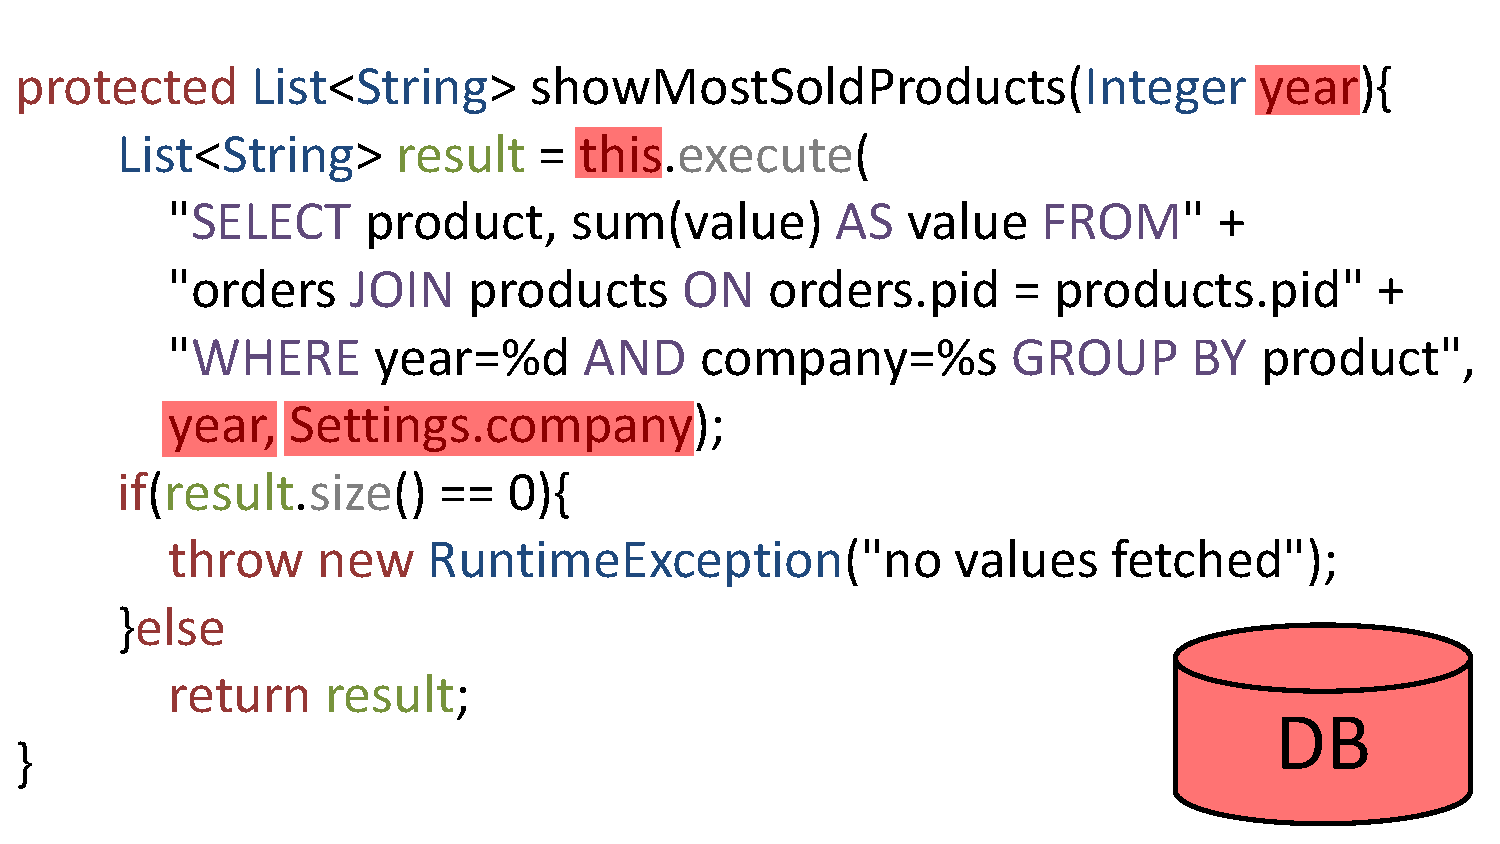
\includegraphics[width=\linewidth]{images/context}
    \caption{Running the statements of this Java method with its embedded SQL query requires the data highlighted in red: the parameter, accessible state, and the database.}
    \label{fig:context_recording}
\end{figure}

When a developer interacts with a specific line in the method's body, one idea would be the use of ordinary breakpoints to establish the necessary runtime data for that specific line of interest. 
Accessible state includes global state and, depending on the used programming language, also state from surrounding scopes, e.g. from surrounding functions.
Snapshots of the database are necessary as methods that embed queries might modify the database, possibly impeding subsequent runs of that method during the interactive development.

We assume the recording approach and method granularity for the remainder of this document.

\subsection{Selecting Data Contexts}

The presented tracing approach generates potentially numerous Data Contexts for each method.
Given our tool traces live systems deployed at customers, each user interaction might lead to recorded data contexts for all triggered executions.
Further, even when our tool only traces deterministic test runs once, particular methods might still be covered through multiple test cases or even be called multiple times in single test cases as, for example, the case with methods called from loops.
For these reasons, a developer might be confronted with many Data Contexts for each statement of interest, when using an implementation of our approach.
Additionally, since Data Contexts from the same trace can be expected to considerably overlap, presenting all of them to the developer might significantly reduce the simplicity, we tried to achieve with our prototype.
Potential approaches to address this issue include automatic selection of interesting samples after clustering all Data Contexts, preselection based on relevance through expert users, or combinations of both methods.
Clustering data contexts could be based on several dimensions, including:
\begin{itemize}
  \item size of the associated database snapshot
  \item control flow that lead to this context
  \item timestamp of this context
\end{itemize}
Nevertheless, even supporting developers with automatic clustering and stored preselections, exploration of the full extent of available contexts would also be desired, in order to make a final decision on which particular Data Context to use during development.
